
\chapter{Advanced Concepts} \label{Advanced}

This chapter discusses some of the more advanced concepts of JavaGroups with respect
to using it and setting it up correctly.



  \section{Setting up the protocol stack}

  This section applies only to the JChannel channel implementation, not to the
  Ensemble or iBus channel implementations.

  When creating a {\tt JChannel}, the properties of the underlying protocol stack can
  be specified as argument. A null argument means use the default composition of
  layers in the protocol stack (which may change between releases of JavaGroups).

  A possible property specification may instruct JavaGroups to create an unreliable,
  UDP-based channel, another one may specify a loss-less, FIFO channel, and yet a
  third one may create a loss-less, FIFO, virtually synchronous, total order channel.

  This section discusses how to create a JChannel with a customized protocol stack
  and the syntax of property strings will be described. It does not describe the
  protocols in detail; see the Programmer's Guide for details. Also, as JavaGroups is
  work in progress, new protocols may be added, or existing ones
  removed/renamed. Refer to the Javadoc documentation for a complete reference.

      
    \subsection{Properties} \label{Properties}

    A property string consists of a number of properties separated by colons:

    \begin{small}
    \begin{verbatim}
    "<prop1>(arg1=val1):<prop2>(arg1=val1;arg2=val2):<prop3>:<propn>"
    \end{verbatim}
    \end{small}

    Each property relates directly to a protocol layer, which is implemented as a
    Java class. When a protocol stack is to be created based on the above property
    string, the first property becomes the bottom-most layer, the second one will be
    placed on the first, etc: the stack is created from the bottom to the top, as the
    string is parsed from left to right. Each property has to be the name of a Java
    class that resides in the {\tt org.jgroups.stack.protocols}
    package\footnote{This package may change in the future.}. Note that only the base
    name has to be given, not the fully specified class name ({\tt UDP} instead of
    {\tt orh.jgroups.stack.protocols.UDP}).

    Each layer may have 0 or more arguments, which are specified as a list of
    name/value pairs in parentheses directly after the property. In the example
    above, the first protocol layer has 1 argument, the second 2, the third
    none. When a layer is created, these properties (if there are any) will be set in
    a layer by invoking the layer's {\tt setProperties()} method\footnote{If in doubt
    what properties are accepted by a layer, this method can always be consulted in
    the source code.}.

    As an example the property string below instructs JavaGroups to create a JChannel
    with protocols {\tt UDP}, {\tt PING}, {\tt FD} and {\tt GMS}:


    \begin{small}
    \begin{verbatim}
    "UDP(mcast_addr=228.10.9.8;mcast_port=5678):PING:FD:GMS"
    \end{verbatim}
    \end{small}


    The {\tt UDP} protocol layer is at the bottom of the stack, and it should use
    mcast address {\tt 228.10.9.8.} and port {\tt 5678} rather than the default IP
    multicast address and port. The only other argument instructs {\tt FD} to output
    debug information while executing. Property {\tt UDP} refers to a class {\tt
    org.jgroups.stack.protocols.UDP}, which is subsequently loaded and an instance
    of which is created as protocol layer. If any of these classes are not found, an
    exception will be thrown and the construction of the stack will be aborted.






  \section{Using multiple channels} \label{MultipleChannels}

  When using a fully virtual synchronous protocol stack, the performance may not be
  great because of the larger number of protocols present. For certain applications,
  however, throughput is more important than ordering, e.g. for video/audio streams
  or airplane tracking. In the latter case, it is important that airplanes are handed
  over between control domains correctly, but if there are a (small) number of radar
  tracking messages (which determine the exact location of the plane) missing, it is
  not a problem. The first type of messages do not occur very often (typically a
  number of messages per hour), whereas the second type of messages would be sent at
  a rate of 10-30 messages/second. The same applies for a distributed whiteboard:
  messages that represent a video or audio stream have to be delivered as quick as
  possible, whereas messages that represent figures drawn on the whiteboard, or new
  participants joining the whiteboard have to be delivered according to a certain
  order.

  The requirements for such applications can be solved by using two separate stacks:
  one for control messages such as group membership, floor control etc and the other
  one for data messages such as video/audio streams (actually one might consider
  using one channel for audio and one for video). The control channel might use
  virtual synchrony, which is relatively slow, but enforces ordering and
  retransmission, and the data channel might use a simple UDP channel, possibly
  including a fragmentation layer, but no retransmission layer (losing packets is
  preferred to costly retransmission).

  The {\tt Draw2Channels} demo program (in the {\tt org.jgroups.demos} package)
  demonstrates how to use two different channels.






  \section{Transport protocols}

  A {\em transport protocol} refers to the protocol at the bottom of the protocol
  stack which is responsible for sending and receiving messages to/from the
  network. There are a number of transport protocols in JavaGroups. They are
  discussed in the following sections.

  A typical protocol stack configuration using UDP is\footnote{Consult the
  Programmer's Guide for details}:

  \begin{small}
  \begin{verbatim}
  "UDP(mcast_addr=224.0.0.35;mcast_port=45566;ip_ttl=32;" +
      "mcast_send_buf_size=150000;mcast_recv_buf_size=80000):" +
  "PING(timeout=2000;num_initial_members=3):" +
  "MERGE2(min_interval=5000;max_interval=10000):" +
  "FD_SOCK:" +
  "VERIFY_SUSPECT(timeout=1500):" +
  "pbcast.STABLE(desired_avg_gossip=20000):" +
  "pbcast.NAKACK(gc_lag=50;retransmit_timeout=300,600,1200,2400,4800):" +
  "UNICAST(timeout=5000;min_wait_time=2000):" +
  "FRAG(frag_size=4096;down_thread=false;up_thread=false):" +
  "pbcast.GMS(join_timeout=5000;join_retry_timeout=2000;" +
              "shun=false;print_local_addr=true)"
  \end{verbatim}
  \end{small}

  In a nutshell the properties of the protocols are:

  \begin{description}
  \item[UDP] Uses IP multicast for group messages and UDP packets for messages to
             individual members
  \item[PING] Uses IP multicast (by default) to find initial members. Once found, the
              current coordinator can be determined and a unicast JOIN request will
              be sent to it
  \item[MERGE2] Will merge subgroups back into one group
  \item[FD\_SOCK] Failure detection based on sockets (in a ring form between
                  members). Generates notification if a member fails
  \item[VERIFY\_SUSPECT] Double-checks whether suspected member is really dead,
                         otherwise suspicion generated from protocol below is discarded
  \item[pbcast.STABLE] Deletes messages that have been seen by all members
                       (distributed message garbage collection)
  \item[pbcast.NAKACK] Ensures (a) message reliability and (b) FIFO. Message
                       reliability guarantees that a message will be received. If
                       not, receiver will request retransmission. FIFO guarantees
                       that all messages from sender P will be received in
                       the order P sent them
  \item[UNICAST] Same as NAKACK for unicast messages: messages from sender P will not
                 be lost (retransmission if necessary) and will be in FIFO order
                (essentially the same as TCP in TCP/IP, without the flow control)
  \item[FRAG] Fragments large messages into smaller ones and reassembles them back at
              the receiver side. For both multicast and unicast messages
  \item[pbcast.GMS] Membership protocol. Responsible for joining/leaving members and
                    installing new views. 
  \end{description}



    \subsection{UDP}

    UDP uses IP multicast for sending messages to all members of a group and UDP
    datagrams for unicast messages (sent to a single member). When started, it opens
    a unicast and multicast socket: the unicast socket is used to send/receive
    unicast messages, whereas the multicast socket sends/receives multicast
    messages. The channel's address will be the address and port number of the {\em
    unicast} socket.


      \subsubsection{Using UDP and plain IP multicasting}

      A protocol stack with UDP as transport protocol is typically used with groups
      whose members run on the same host or are distributed across a LAN. Before
      running such a stack a programmer has to ensure that IP multicast is enabled
      across subnets. It is often the case that IP multicast is not enabled across
      subnets. Refer to section \ref{ItDoesntWork} for running a test program that
      determines whether members can reach each other via IP multicast. If this does
      not work, the protocol stack cannot use UDP with IP multicast as transport. In
      this case, the stack has to either use UDP without IP multicasting or other
      transports such as TCP.



      \subsubsection{Using UDP without IP multicasting} \label{IpNoMulticast}

      The protocol stack with UDP and PING as the bottom protocols use IP
      multicasting by default to send messages to all members (UDP) and for discovery
      of the initial members (PING). However, if multicasting cannot be used, the UDP
      and PING protocols can be configured to send multiple unicast messages instead
      of one multicast message\footnote{Although not as efficient (and using more
      bandwidth), it is sometimes the only possibility to reach group members.} (UDP)
      and to access a well-known server ({\em GossipServer}) for initial membership
      information (PING).

      To configure UDP to use multiple unicast messages to send a group message
      instead of using IP multicasting, the {\tt ip\_mcast} property has to be set to
      {\tt false}.

      To configure PING to access a GossipServer instead of using IP multicast the
      following properties have to be set:

      \begin{description}
      \item[gossip\_host] The name of the host on which GossipServer is started
      \item[gossip\_port] The port on which GossipServer is listening
      \item[gossip\_refresh] The number of milliseconds to wait until refreshing our
                             address entry with the GossipServer
      \end{description}

      Before any members are started the GossipServer has to be started, e.g.

      {\tt java org.jgroups.stack.GossipServer -port 5555}.

      This starts the GossipServer on the local host on port 5555. The GossipServer
      is essentially a lookup service for groups and members. It is a process that
      runs on a well-known host and port and accepts GET(group) and REGISTER(group,
      member) requests. The REGISTER request registers a member's address and group
      with the GossipServer. The GET request retrieves all member addresses given a
      group name. Each member has to periodically ({\tt gossip\_refresh}) re-register
      their address with the GossipServer, otherwise the entry for that member will be
      removed (accommodating for crashed members).

      The following example shows how to disable the use of IP multicasting and use a
      GossipServer instead. Only the bottom two protocols are shown, the rest of the
      stack is the same as in the previous example:

      \begin{small}
      \begin{verbatim}
      "UDP(ip_mcast=false;mcast_addr=224.0.0.35;mcast_port=45566;ip_ttl=32;" +
          "mcast_send_buf_size=150000;mcast_recv_buf_size=80000):" +
      "PING(gossip_host=localhost;gossip_port=5555;gossip_refresh=15000;" +
           "timeout=2000;num_initial_members=3):" +
      \end{verbatim}
      \end{small}

      The property {\tt ip\_mcast} is set to {\tt false} in {\tt UDP} and the gossip
      properties in {\tt PING} define the GossipServer to be on the local host at
      port 5555 with a refresh rate of 15 seconds. If PING is parameterized with the
      GossipServer's address {\em and} port, then gossiping is enabled, otherwise it
      is disabled. If only one parameter is given, gossiping will be {\em disabled}.

      Make sure to run the GossipServer before starting any members, otherwise the
      members will not find each other and each member will form its own
      group\footnote{This can actually be used to test the MERGE2 protocol: start two
      members (forming two singleton groups because they don't find each other), then
      start the GossipServer. After some time, the two members will merge into one
      group}.
       






    \subsection{TCP}

    TCP is a replacement of UDP as bottom layer in cases where IP Multicast based on
    UDP is not desired. This may be the case when operating over a WAN, where routers
    will discard IP MCAST. As a rule of thumb UDP is used as transport for LANs,
    whereas TCP is used for WANs.

    The properties for a typical stack based on TCP might look like this:

    \begin{small}
    \begin{verbatim}
    "TCP(start_port=7800):" +
    "TCPPING(initial_hosts=localhost[7800];port_range=5;timeout=3000;" +
            "num_initial_members=3;up_thread=true;down_thread=true):" +
    "VERIFY_SUSPECT(timeout=1500;down_thread=false;up_thread=false):" +
    "pbcast.STABLE(desired_avg_gossip=20000;down_thread=false;up_thread=false):" +
    "pbcast.NAKACK(down_thread=true;up_thread=true;gc_lag=100;retransmit_timeout=3000):" +
    "pbcast.GMS(join_timeout=5000;join_retry_timeout=2000;shun=false;" +
               "print_local_addr=false;down_thread=true;up_thread=true)";
    \end{verbatim}
    \end{small}


    \begin{description}
    \item[TCP] The transport protocol, uses TCP (from TCP/IP) to send unicast and
               multicast messages. In the latter case, it sends multiple unicast
               messages.
    \item[TCPPING] Discovers the initial membership to determine coordinator. Join
                   request will then be sent to coordinator.
    \item[VERIFY\_SUSPECT] Double checks that a suspected member is really dead
    \item[pbcast.STABLE] Distributed garbage collection of messages seen by all
                         members
    \item[pbcast.NAKACK] Reliable and FIFO message delivery
    \item[pbcast.GMS] Membership services. Takes care of joining and removing new/old
                      members, emits view changes
    \end{description}

	   
    Since TCP already offers some of the reliability guarantees that UDP doesn't,
    some protocols (e.g. FRAG and UNICAST) are not needed on top of TCP.

    When using TCP, each message to the group is sent as multiple unicast messages
    (one to each member). Due to the fact that IP multicasting cannot be used to
    discover the initial members, another mechanism has to be used to find the
    initial membership. There are a number of alternatives:

    \begin{enumerate}
    \item PING with GossipServer: same solution as described in
          \ref{IpNoMulticast}. The {\tt ip\_mcast} property has to be set to {\tt
          false}. GossipServer has to be started before the first member is started.
    \item TCPPING: uses a list of well-known group members that it solicits for
                   initial membership
    \item TCPGOSSIP: essentially the same as the above PING\footnote{PING and
                     TCPGOSSIP will be merged in the future.}. The only difference is
                     that TCPGOSSIP allows for multiple GossipServers instead of only
                     one.
    \end{enumerate}

    The next two section illustrate the use of TCP with both TCPPING and TCPGOSSIP.




      \subsubsection{Using TCP and TCPPING}
      
      A protocol stack using TCP and TCPPING looks like this (other protocol
      omitted):

      \begin{small}
      \begin{verbatim}
      "TCP(start_port=7800):" +
      "TCPPING(initial_hosts=HostA[7800],HostB[7800];port_range=5;timeout=3000;" +
               "num_initial_members=3;up_thread=true;down_thread=true):" +
      \end{verbatim}
      \end{small}
      
      The concept behind TCPPING is that no external daemon such as GossipServer is
      needed. Instead some selected group members assume the role of well-known hosts
      from which initial membership information can be retrieved. In the example {\tt
      HostA} and {\tt HostB} are designated members that will be used by TCPPING to
      lookup the initial membership. The property {\tt start\_port} in {\tt TCP}
      means that each member should try to assign port 7800 for itself. If this is
      not possible it will try the next higher port ({\tt 7801}) and so on, until it
      finds an unused port.
      
      {\tt TCPPING} will try to contact both {\tt HostA} and {\tt HostB}, starting at
      port {\tt 7800} and ending at port {\tt 7800 + port\_range}, in the above
      example ports {\tt 7800} - {\tt 7804}. Assuming that at least one of {\tt
      HostA} or {\tt HostB} is up, a response will be received. To be absolutely sure
      to receive a response all the hosts on which members of the group will be
      running can be added to the configuration string.




      \subsubsection{Using TCP and TCPGOSSIP}

      As mentioned before {\tt TCPGOSSIP} is essentially the same as {\tt PING} with
      properties {\tt gossip\_host}, {\tt gossip\_port} and {\tt gossip\_refresh}
      set. However, in TCPGOSSIP these properties are called differently as shown
      below (only the bottom two protocols are shown):

      \begin{small}
      \begin{verbatim}
      "TCP:" +
      "TCPGOSSIP(initial_hosts=localhost[5555],localhost[5556];gossip_refresh_rate=10000;" +
                 "num_initial_members=3;up_thread=true;down_thread=true):" +
      \end{verbatim}
      \end{small}
      
      The {\tt initial\_hosts} properties combines both the host and port of a
      GossipServer, and it is possible to specify more than one GossipServer. In the
      example there are two GossipServers at ports {\tt 5555} and {\tt 5556} on the
      local host. Also, {\tt gossip\_refresh\_rate} defines how many milliseconds to
      wait between refreshing the entry with the GossipServers.

      The advantage of having multiple GossipServers is that, as long as at least one
      is running, new members will always be able to retrieve the initial
      membership. Note that the GossipServer should be started before any of the
      members.




    \subsection{TUNNEL}


      \subsubsection{Using TUNNEL to tunnel a firewall}

      Firewalls are usually placed at the connection to the internet. They shield
      local networks from outside attacks by screening incoming traffic and rejecting
      connection attempts to host inside the firewalls by outside machines. Most
      firewall systems allow hosts inside the firewall to connect to hosts outside it
      (outgoing traffic), however, incoming traffic is most often disabled entirely.

      {\em Tunnels} are host protocols which encapsulate other protocols by
      multiplexing them at one end and demultiplexing them at the other end. Any
      protocol can be tunneled by a tunnel protocol.

      The most restrictive setups of firewalls usually disable {\em all} incoming
      traffic, and only enable a few selected ports for outgoing traffic. In the
      solution below, it is assumed that 2 TCP ports are enabled for outgoing ports;
      one for the GossipServer and one for the Router.

      JavaGroups has a mechanism that allows a programmer to tunnel a firewall. The
      solution involves a GossipServer and a Router process. Both have to be outside
      of the firewall, so other members (possibly also behind firewalls) can access
      it.

      The solution works as follows. A channel inside a firewall has to use protocol
      TUNNEL instead of UDP as bottommost layer in the stack, plus either PING or
      TCPGOSSIP, as shown below (only the bottom two protocols shown):

      \begin{small}
      \begin{verbatim}
      "TUNNEL(router_host=localhost;router_port=12001):" +
      "TCPGOSSIP(initial_hosts=localhost[12002];gossip_refresh_rate=10000;" +
                 "num_initial_members=3;up_thread=true;down_thread=true):"
      \end{verbatim}
      \end{small}
      
      {\tt TCPGOSSIP} uses the GossipServer (outside the firewall) at port {\tt
      12002} to register its address (periodically) and to retrieve the initial
      membership for its group.

      {\tt TUNNEL} establishes a TCP connection to a {\em Router} process (also
      outside the firewall) that accepts messages from members and passes them on to
      other members. This connection is initiated by the host inside the firewall and
      persists as long as the channel is connected to a group. Router will use the
      {\em same connection} to send incoming messages to the channel that initiated
      the connection. This is perfectly legal, as TCP connections are fully
      duplex. Note that, if Router tried to establish its own TCP connection to the
      channel behind the firewall, it would fail. But it is okay to reuse the
      existing TCP connection, established by the channel.

      Note that {\tt TUNNEL} has to be given the hostname and port of the Router
      process. This example assumes a Router is running on the local host at port
      {\tt 12001} and a GossipServer is running at port {\tt 12002}.

      Any time a message has to be sent, TUNNEL forwards the message to Router, which
      distributes it to its destination: if the message's destination field is null
      (send to all group members), then Router looks up the members that belong to
      that group and forwards the message to all of them via the TCP connection they
      established when connecting to Router. If the destination is a valid member
      address, then that member's TCP connection is looked up, and the message is
      forwarded to it\footnote{To do so, Router has to maintain a table between
      groups, member addresses and TCP connections.}.

      To tunnel a firewall using JavaGroups, the following steps have to be taken:

      \begin{enumerate}

      \item Check that 2 TCP ports (e.g. 12001 and 12002) are enabled in the firewall
            for outgoing traffic
      \item Start the GossipServer:
        \begin{small}
	\begin{verbatim}
        start org.jgroups.stack.GossipServer -port 12002
      \end{verbatim}
      \end{small}


      \item Start Router:
        \begin{small}
	\begin{verbatim}
        java org.jgroups.stack.Router -port 12001
      \end{verbatim}
      \end{small}


      \item Configure the TUNNEL protocol layer as instructed above.

      \item Create a channel

      \end{enumerate}


      The general setup is shown in fig. \ref{TunnelingFig}.

      \begin{figure}[htb]
      \center{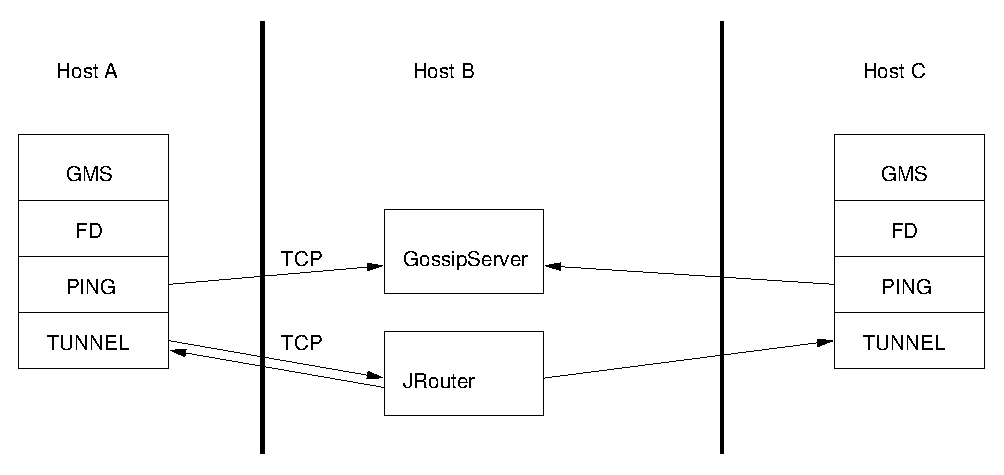
\epsfig{file=figs/Tunneling.eps,width=.65\textwidth}}
      \caption{Tunneling a firewall}
      \label{TunnelingFig}
      \end{figure}

      First, the GossipServer and Router processes are created on host B. Note that
      these should be outside the firewall, and all channels in the same group should
      use the same GossipServer and Router processes. When a channel on host A is
      created, its {\tt TCPGOSSIP} protocol will register its address with the
      GossipServer and retrieve the initial membership (assume this is C). Now, a TCP
      connection with Router is established by A; this will persist until A crashes
      or voluntarily leaves the group. When A multicasts a message to the group,
      Router looks up all group members (in this case, A and C) and forwards the
      message to all members, using their TCP connections. In the example, A would
      receive its own copy of the multicast message it sent, and another copy would
      be sent to C.
	
      This scheme allows for example {\em Java applets}, which are only allowed to
      connect back to the host from which they were downloaded, to use JavaGroups:
      the HTTP server would be located on host B and the gossip and Router daemons
      would also run on that host. An applet downloaded to either A or C would be
      allowed to make a TCP connection to B. Also, applications behind a firewall
      would be able to talk to each other, joining a group.

      However, there are several drawbacks: first, the central GossipServer and Router
      processes constitute a single point of failure (if host B
      crashes)\footnote{Although multiple GossipServer could be started}, second,
      having to maintain a TCP connection for the duration of the connection might
      use up resources in the host system (e.g. in the Router), leading to
      scalability problems, third, this scheme is inappropriate when only a few
      channels are located behind firewalls, and the vast majority can indeed use IP
      multicast to communicate, and finally, it is not always possible to enable
      outgoing traffic on 2 ports in a firewall, e.g. when a user does not 'own' the
      firewall.


    \subsection{Difference between Router and GossipServer}
    
    The Router and GossipServer processes have overlapping functionality: both of
    them allows a member to fetch initial membership information. In addition the
    Router provides routing functionality. The reason for not merging the
    functionalities is that some (probably most) applications only need gossiping,
    but not routing functionality. Therefore they will use the lightweight
    GossipServer, without having to use Router whose routing functionality would not
    be used. As a matter of fact both processes used to be merged in earlier versions
    of JavaGroups.



